% !TeX program = xelatex

\documentclass{article}
\usepackage{sarcastikz}
\usepackage{fontspec}
\newfontfamily{\comicfont}{Gloria Hallelujah}
\setmainfont{Roboto}
\usepackage[landscape]{geometry}
\usetikzlibrary{calc,decorations.pathmorphing,patterns, backgrounds}
\newcounter{comiccount}
\stepcounter{comiccount}

\makeatletter

\pgfdeclaredecoration{penciline}{initial}{
	\state{initial}[width=+\pgfdecoratedinputsegmentremainingdistance,auto corner on length=1mm,]{
		\pgfpathcurveto%
		{% From
			\pgfqpoint{\pgfdecoratedinputsegmentremainingdistance}
			{\pgfdecorationsegmentamplitude}
		}
		{%  Control 1
			\pgfmathrand
			\pgfpointadd{\pgfqpoint{\pgfdecoratedinputsegmentremainingdistance}{0pt}}
			{\pgfqpoint{-\pgfdecorationsegmentaspect\pgfdecoratedinputsegmentremainingdistance}%
				{\pgfmathresult\pgfdecorationsegmentamplitude}
			}
		}
		{%TO 
			\pgfpointadd{\pgfpointdecoratedinputsegmentlast}{\pgfpoint{1pt}{1pt}}
		}
	}
	\state{final}{}
}
\makeatother

\newenvironment{comics}{%
	\section*{{\Huge sarcasTikz }- grad school in \LaTeX}%
	\begin{center}%
}
{%
	
\thecomiccount - Adarsh
\end{center}%
\stepcounter{comiccount}
}

\newcommand\newdummy[2][]{\begin{scope}[#2] 
\dummy[#1]
\end{scope}}
% colors
\definecolor{skycolor}{HTML}{87CEFA}
\begin{document}
	

\begin{comics}
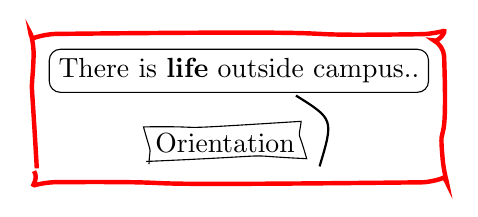
\begin{tikzpicture}[framed, scale=0.6, decoration=penciline, background rectangle/.style={ultra thick,draw=red, rounded corners, decorate}]
\begin{scope}
\node[rectangle,draw, decorate] at (3.5,3.5) {\comicfont Orientation};
\draw[thick] (5.5, 3) .. controls (5.8, 4) .. (5, 4.5);
\node[rectangle, rounded corners, draw] at ([yshift=0.5cm]current bounding box.north) {There is {\bf life} outside campus..};
\end{scope}

\begin{scope}
\dummy[tshirt=black, pant=blue!40!green, shoe, boyhair, viewright, normal]
\end{scope}

\begin{scope}[xshift=4cm]
\dummy[pupil=green, tomhair, hair=brown, tshirt=white, pant=blue, shoe=brown, viewleft, speak]
\end{scope}
\end{tikzpicture}
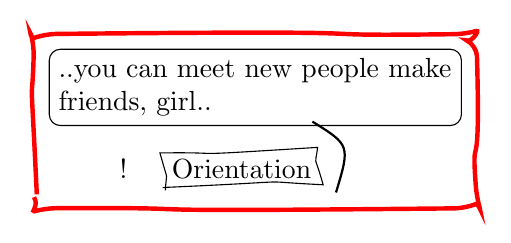
\begin{tikzpicture}[framed, scale=0.6, decoration=penciline, background rectangle/.style={ultra thick,draw=red, rounded corners, decorate}]
\begin{scope}
\node[rectangle,draw, decorate] at (3.5,3.5) {\comicfont Orientation};
\draw[thick] (5.5, 3) .. controls (5.8, 4) .. (5, 4.5);
\node[rectangle, rounded corners, draw, text width = 5cm] at ([yshift=0.7cm]current bounding box.north) {..you can meet new people make friends, girl..};
\node[] at (1,3.5) {!};
\end{scope}

\begin{scope}
\dummy[tshirt=black, pant=blue!40!green, shoe, boyhair, poker]
\end{scope}

\begin{scope}[xshift=4cm]
\dummy[pupil=green, tomhair, hair=brown, tshirt=white, pant=blue, shoe=brown, viewleft, speak]
\end{scope}
\end{tikzpicture}
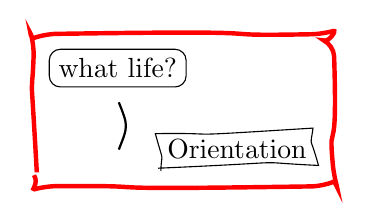
\begin{tikzpicture}[framed, scale=0.6, decoration=penciline, background rectangle/.style={ultra thick,draw=red, rounded corners, decorate}]
\begin{scope}
\node[rectangle,draw, decorate] at (3.5,3.5) {\comicfont Orientation};
\draw[thick] (1, 3.5) .. controls (1.2, 4) .. (1, 4.5);
\node[rectangle, rounded corners, draw] at ([yshift=0.7cm]current bounding box.north west) {what life?};
\end{scope}

\begin{scope}
\dummy[tshirt=black, pant=blue!40!green, shoe, boyhair, viewright, speak]
\end{scope}

\begin{scope}[xshift=4cm]
\dummy[pupil=green, tomhair, hair=brown, tshirt=white, pant=blue, shoe=brown, poker]
\end{scope}
\end{tikzpicture}
\end{comics}

%% Eclipse
\begin{comics}
	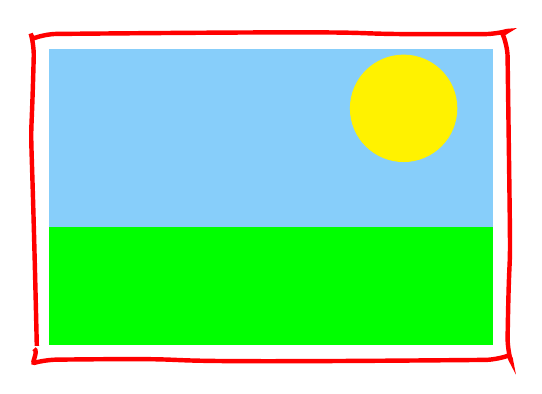
\begin{tikzpicture}[framed, scale=0.75, decoration=penciline, background rectangle/.style={ultra thick,draw=red, rounded corners, decorate}]
	\begin{scope}
	\filldraw[green](-2,0) rectangle (5.5,2);
	\filldraw[skycolor](-2,2) rectangle (5.5,5);
	\filldraw[yellow] (4,4) circle (0.9cm);
	\end{scope}
	
	\begin{scope}
	\dummy[tshirt=black, pant=blue!40!green, shoe, boyhair, normal]
	\end{scope}
	\end{tikzpicture}
	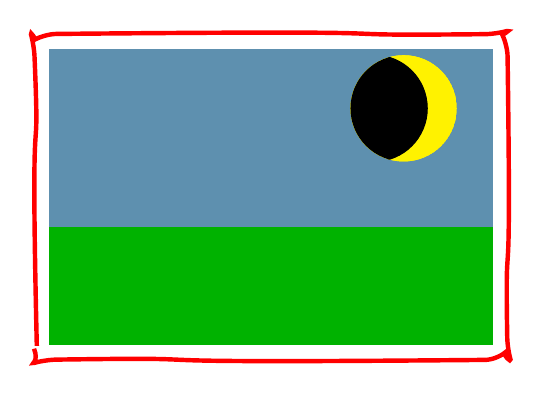
\begin{tikzpicture}[framed, scale=0.75, decoration=penciline, background rectangle/.style={ultra thick,draw=red, rounded corners, decorate}]
	\begin{scope}
	\filldraw[green!70!black](-2,0) rectangle (5.5,2);
	\filldraw[skycolor!70!black](-2,2) rectangle (5.5,5);
	\clip (4,4) circle (0.9cm);
	\filldraw[yellow] (4,4) circle (0.9cm);
	\filldraw[black] (3.5,4) circle (0.9cm);
	\end{scope}
	\newdummy[girlhair, hair=black, body=black!30!brown, paperglass]{xshift=-1.2cm, yshift=2cm,scale=0.8}
	\newdummy[tomhair, hair=brown, paperglass]{xshift=0.8cm, yshift=2cm,scale=0.8}
	\newdummy[tomhair, hair=white, tshirt=red, pant=blue, pupil=yellow, paperglass]{xshift=-2cm}
	\newdummy[paperglass, girlhair, hair=brown!50!black, tshirt=blue, pant=black, pupil=green]{xshift=2cm}
	%\begin{scope}
	\newdummy[tshirt=black, pant=blue!40!green, shoe, boyhair]{}
	%\end{scope}
	\end{tikzpicture}
	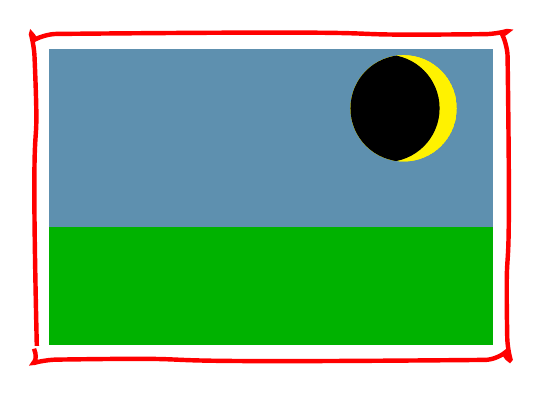
\begin{tikzpicture}[framed, scale=0.75, decoration=penciline, background rectangle/.style={ultra thick,draw=red, rounded corners, decorate}]
	\begin{scope}
	\filldraw[green!70!black](-2,0) rectangle (5.5,2);
	\filldraw[skycolor!70!black](-2,2) rectangle (5.5,5);
	\clip (4,4) circle (0.9cm);
	\filldraw[yellow] (4,4) circle (0.9cm);
	\filldraw[black] (3.7,4) circle (0.9cm);
	\end{scope}
	\newdummy[girlhair, hair=black, body=black!30!brown, paperglass]{xshift=-1.2cm, yshift=2cm,scale=0.8}
	\newdummy[tomhair, hair=brown, paperglass]{xshift=0.8cm, yshift=2cm,scale=0.8}
	\newdummy[tomhair, hair=white, tshirt=red, pant=blue, pupil=yellow, paperglass]{xshift=-2cm}
	\newdummy[paperglass, girlhair, hair=brown!50!black, tshirt=blue, pant=black, pupil=green]{xshift=2cm}
	%\begin{scope}
	\newdummy[tshirt=black, pant=blue!40!green, shoe, boyhair, paperglass, smile]{}
	%\end{scope}
	\end{tikzpicture}
\end{comics}

%% supreme court judgement
\begin{comics}
	
\begin{tikzpicture}
	\node[](a){};
	\node[below] at (a) {\comicfont Meanwhile in India..};
	\end{tikzpicture}
	
	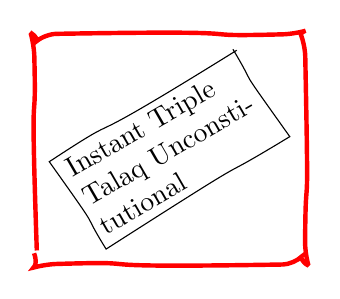
\begin{tikzpicture}[framed, scale=0.9, decoration=penciline, background rectangle/.style={ultra thick,draw=red, rounded corners, decorate}]
	\begin{scope}
	\node[draw=black, rectangle, decorate, minimum width=2.5cm, text width=2.5cm, rotate=30] at (0, 3.5) {\comicfont Instant Triple Talaq Unconstitutional}; 
	\end{scope}
	\newdummy[judge, shoe=blue!40!black, pupil=green!50!black, lawhammer, judgehair, hair=white, poker]{}
	\end{tikzpicture}
	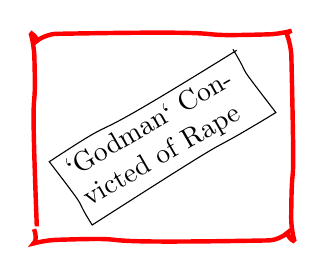
\begin{tikzpicture}[framed, scale=0.9, decoration=penciline, background rectangle/.style={ultra thick,draw=red, rounded corners, decorate}]
	\begin{scope}
	\node[draw=black, rectangle, decorate, minimum width=2.5cm, text width=2.5cm, rotate=30] at (0, 3.5) {\comicfont `Godman` Convicted of Rape}; 
	\end{scope}
	\newdummy[judge, shoe=blue!40!black, pupil=green!50!black, lawhammer, judgehair, hair=white]{}
	\end{tikzpicture}
	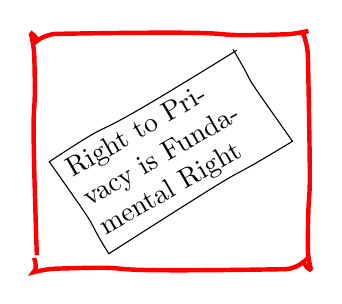
\begin{tikzpicture}[framed, scale=0.9, decoration=penciline, background rectangle/.style={ultra thick,draw=red, rounded corners, decorate}]
	\begin{scope}
	\node[draw=black, rectangle, decorate, minimum width=2.5cm, text width=2.5cm, rotate=30] at (0, 3.5) {\comicfont Right to Privacy is Fundamental Right}; 
	\end{scope}
	\newdummy[judge, shoe=blue!40!black, pupil=green!50!black, lawhammer, judgehair, hair=white, smile]{}
	\end{tikzpicture}
\end{comics}

\pagebreak
%% purdue construction
\begin{comics}
	
\begin{tikzpicture}
	\node[](a){};
	\node[below] at (a) {\comicfont Meanwhile at Purdue..};
	\end{tikzpicture}
	
	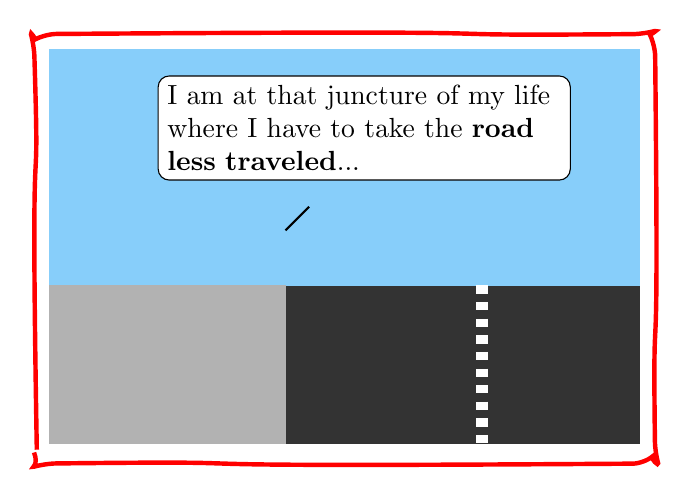
\begin{tikzpicture}[framed, decoration=penciline, background rectangle/.style={ultra thick,draw=red, rounded corners, decorate}]
	\begin{scope}
	\filldraw[white!20!black](-2,0) rectangle (5.5,2);
	\filldraw[skycolor](-2,2) rectangle (5.5,5);
	\draw[dashed, line width=1.5mm, white] (3.5, 2) -- (3.5, 0);
	\filldraw[white!70!black](-2,0) rectangle (1,2);
	\node[rectangle,fill= white, rounded corners, draw, text width=5cm] at (2, 4) {I am at that juncture of my life where I have to take the {\bf road less traveled}...};
	\draw[thick] (1, 2.7) -- (1.3, 3);
	\end{scope}
	
	\begin{scope}
	\newdummy[tshirt=black, pant=blue!40!green, shoe, boyhair, normal]{xshift=-2cm}
	\end{scope}
	\end{tikzpicture}
	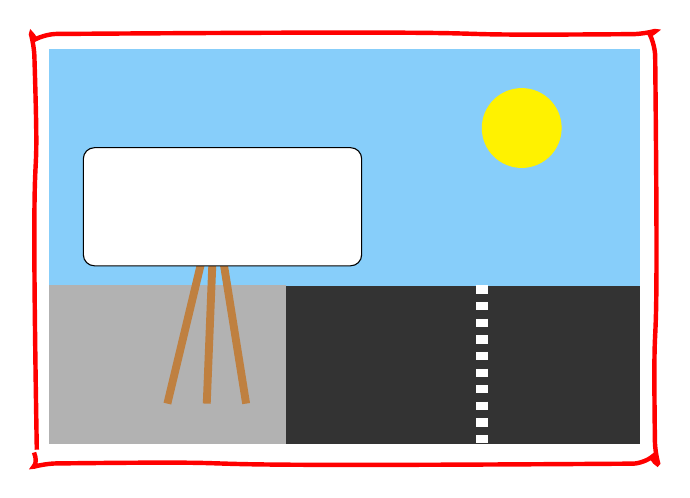
\begin{tikzpicture}[framed, decoration=penciline, background rectangle/.style={ultra thick,draw=red, rounded corners, decorate}]
	\begin{scope}
	\filldraw[white!20!black](-2,0) rectangle (5.5,2);
	\filldraw[skycolor](-2,2) rectangle (5.5,5);
	\filldraw[yellow] (4,4) circle (0.5cm);
	\draw[dashed, line width=1.5mm, white] (3.5, 2) -- (3.5, 0);
	\filldraw[white!70!black](-2,0) rectangle (1,2);
	\draw[brown, line width=1mm] (-0.5, 0.5) -- (0.1, 3) -- (0.5, 0.5);
	\draw[brown, line width=1mm] (0.1, 3) -- (0, 0.5);
	\node[rectangle,fill= orange!70!red, white, rounded corners, draw=black, text width=3.3cm, minimum height=1.5cm] at (0.2, 3) {\bf Construction Ahead. \phantom{aa}$\leftarrow$ DETOUR};
	\end{scope}
	\end{tikzpicture}
\end{comics}

\end{document}